% Generative Compression for Differentiable Opaque Meshes -- technical report
% VERSION: report-latex-v2 (2026-11-03): byte prices B_a / B_f (additive only), split/prune worked-example figure, cross-method table split in two. Compile with pdflatex (Overleaf default works).
\documentclass[11pt,a4paper]{article}
\usepackage[margin=2.2cm]{geometry}
\usepackage[T1]{fontenc}
\usepackage[utf8]{inputenc}
\usepackage{lmodern}
\usepackage{amsmath,amssymb}
\usepackage{graphicx}
\usepackage{booktabs}
\usepackage{array}
\usepackage{xcolor}
\usepackage{caption}
\usepackage{tikz}
\usetikzlibrary{arrows.meta,positioning,calc,fit}
\usepackage{enumitem}
\usepackage[colorlinks=true,linkcolor=blue!60!black,citecolor=blue!60!black,urlcolor=blue!60!black]{hyperref}

\captionsetup{font=small,labelfont=bf}
\definecolor{ours}{RGB}{31,119,80}
\definecolor{oursfill}{RGB}{229,243,236}
\definecolor{edge}{RGB}{90,90,90}
\definecolor{quiet}{RGB}{110,110,110}

\newcommand{\MB}{\,\mathrm{MB}}
\newcommand{\dB}{\,\mathrm{dB}}

\title{Generative Compression for Differentiable Opaque Meshes\\[2pt]
\large Technical report}

\begin{document}
\maketitle

\begin{abstract}
MeshSplatting produces an opaque, engine-ready triangle mesh with per-vertex spherical harmonics (SH), but its FP32 output is 430--740\,MB per scene. We keep MeshSplatting's optimisation untouched and add two training-time decisions and one delivery codec: triangles are split only when the distortion they remove is worth the bytes they add, the same price is applied in reverse as an edge-collapse prune, and the trained mesh is encoded into a single file whose per-vertex SH is replaced by shared dictionary indices. One rate--distortion parameter $\lambda$ traces the whole curve. On Mip-NeRF~360 the 642\,MB FP32 mesh becomes 26.6\,MB at $-0.24$\,dB (24$\times$), 9.0\,MB at $-0.92$\,dB (72$\times$) and 4.3\,MB at $-1.68$\,dB (151$\times$); the delivered asset is a standard mesh that decodes in 2--6\,s on one CPU core and renders at 145--350\,fps on a phone.
\end{abstract}

% =====================================================================
\section{Methodology}
\label{sec:method}

We keep MeshSplatting's optimisation untouched and change two things: \emph{which} triangles get split during growth (priced in bytes), and a reverse prune under the same price. The trained mesh then goes through a codec that replaces per-vertex SH by shared dictionary indices. The vertex count is no longer a hand-set cap but an output of one rate--distortion trade-off $\lambda$. Figure~\ref{fig:pipeline} shows where the pieces sit.

\begin{figure}[t]
\centering
\resizebox{\linewidth}{!}{%
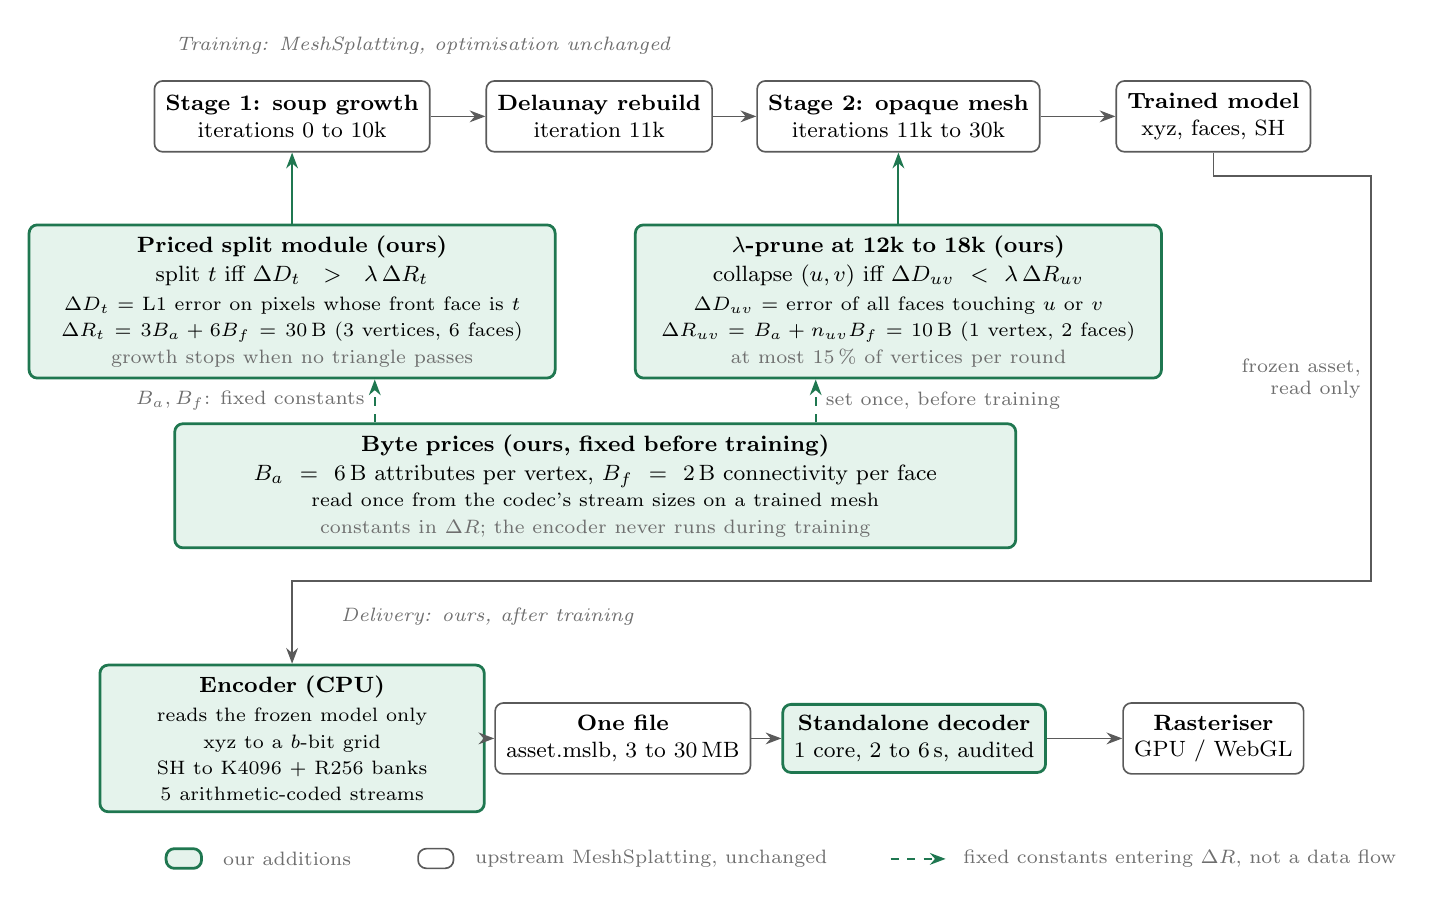
\begin{tikzpicture}[
  font=\footnotesize,
  >={Stealth[length=2mm]},
  up/.style={draw=edge, rounded corners=3pt, line width=0.6pt, align=center, inner sep=4pt, minimum height=9mm},
  ourbox/.style={draw=ours, fill=oursfill, rounded corners=3pt, line width=1.0pt, align=center, inner sep=4pt},
  flow/.style={->, draw=edge, line width=0.6pt},
  ourflow/.style={->, draw=ours, line width=0.7pt},
  price/.style={->, draw=ours, dashed, line width=0.7pt},
  lane/.style={font=\scriptsize\itshape, text=quiet},
  body/.style={font=\scriptsize, text=black},
]
% ---- lane 1: upstream training
\node[lane, anchor=west] at (0,0.9) {Training: MeshSplatting, optimisation unchanged};
\node[up] (s1) at (1.6,0) {\textbf{Stage 1: soup growth}\\ iterations 0 to 10k};
\node[up] (del) at (5.5,0) {\textbf{Delaunay rebuild}\\ iteration 11k};
\node[up] (s2) at (9.3,0) {\textbf{Stage 2: opaque mesh}\\ iterations 11k to 30k};
\node[up] (model) at (13.3,0) {\textbf{Trained model}\\ xyz, faces, SH};
\draw[flow] (s1) -- (del);
\draw[flow] (del) -- (s2);
\draw[flow] (s2) -- (model);

% ---- lane 2: our priced decisions
\node[ourbox, below=9mm of s1.south, anchor=north, text width=6.4cm] (split) {
  \textbf{Priced split module (ours)}\\[1pt]
  split $t$ iff $\Delta D_t > \lambda\,\Delta R_t$\\[1pt]
  {\scriptsize $\Delta D_t$ = L1 error on pixels whose front face is $t$}\\
  {\scriptsize $\Delta R_t = 3B_a + 6B_f = 30$\,B (3 vertices, 6 faces)}\\
  {\scriptsize\color{quiet} growth stops when no triangle passes}};
\node[ourbox, below=9mm of s2.south, anchor=north, text width=6.4cm] (prune) {
  \textbf{$\lambda$-prune at 12k to 18k (ours)}\\[1pt]
  collapse $(u,v)$ iff $\Delta D_{uv} < \lambda\,\Delta R_{uv}$\\[1pt]
  {\scriptsize $\Delta D_{uv}$ = error of all faces touching $u$ or $v$}\\
  {\scriptsize $\Delta R_{uv} = B_a + n_{uv}B_f = 10$\,B (1 vertex, 2 faces)}\\
  {\scriptsize\color{quiet} at most 15\,\% of vertices per round}};
\draw[ourflow] (split.north) -- (s1.south);
\draw[ourflow] (prune.north) -- (s2.south);

% ---- price table
\node[ourbox, text width=10.4cm] (price) at ($(split.south)!0.5!(prune.south) + (0,-1.35)$) {
  \textbf{Byte prices (ours, fixed before training)}\\[1pt]
  $B_a = 6$\,B attributes per vertex, $B_f = 2$\,B connectivity per face\\
  {\scriptsize read once from the codec's stream sizes on a trained mesh}\\
  {\scriptsize\color{quiet} constants in $\Delta R$; the encoder never runs during training}};
\draw[price] ([xshift=-2.8cm]price.north) -- ([xshift=-2.8cm]price.north |- split.south) node[midway, left, body, text=quiet] {$B_a, B_f$: fixed constants};
\draw[price] ([xshift=2.8cm]price.north) -- ([xshift=2.8cm]price.north |- prune.south) node[midway, right, body, text=quiet] {set once, before training};

% ---- lane 3: delivery
\node[lane, anchor=west] at (2.1,-6.35) {Delivery: ours, after training};
\node[ourbox, text width=4.6cm] (enc) at (1.6,-7.9) {
  \textbf{Encoder (CPU)}\\[1pt]
  {\scriptsize reads the frozen model only}\\
  {\scriptsize xyz to a $b$-bit grid}\\
  {\scriptsize SH to K4096 + R256 banks}\\
  {\scriptsize 5 arithmetic-coded streams}};
\node[up] (file) at (5.8,-7.9) {\textbf{One file}\\ asset.mslb, 3 to 30\,MB};
\node[ourbox] (dec) at (9.5,-7.9) {\textbf{Standalone decoder}\\ 1 core, 2 to 6\,s, audited};
\node[up] (ras) at (13.3,-7.9) {\textbf{Rasteriser}\\ GPU / WebGL};
\draw[flow] (enc) -- (file);
\draw[flow] (file) -- (dec);
\draw[flow] (dec) -- (ras);
\draw[flow] (model.south) -- ++(0,-0.3) -| (15.3,-5.9) node[pos=0.75, left, body, text=quiet, align=right] {frozen asset,\\ read only} -- (1.6,-5.9) -- (enc.north);

% ---- key
\begin{scope}[shift={(0,-9.55)}]
\draw[ourbox, minimum width=4mm, minimum height=2.5mm] (0,0) rectangle (0.45,0.25);
\node[body, text=quiet, anchor=west] at (0.6,0.12) {our additions};
\draw[up, minimum width=4mm] (3.2,0) rectangle (3.65,0.25);
\node[body, text=quiet, anchor=west] at (3.8,0.12) {upstream MeshSplatting, unchanged};
\draw[price] (9.2,0.12) -- (9.9,0.12);
\node[body, text=quiet, anchor=west] at (10.0,0.12) {fixed constants entering $\Delta R$, not a data flow};
\end{scope}
\end{tikzpicture}}
\caption{Pipeline: two priced decisions during training, one dictionary codec at delivery. Grey boxes are MeshSplatting as published; tinted boxes are ours. The byte prices are two constants read once from the codec's stream sizes; the encoder itself runs only on the frozen, finished model and cannot influence how the mesh grew.}
\label{fig:pipeline}
\end{figure}

\subsection{Where we intervene in MeshSplatting}

Upstream training has two stages. \textbf{Stage 1 (iterations 0--10\,000)} grows a soft triangle soup: every 500 iterations a fixed fraction of triangles (\texttt{add\_percentage}) is split, chosen by importance sampling, up to a hand-set cap. At iteration 11\,000 a restricted Delaunay rebuild re-triangulates the soup. \textbf{Stage 2 (11\,000--30\,000)} optimises the now-opaque mesh (opacity schedule, $2\times$/$4\times$ supersampling after 20k/25k).

Our changes sit only in the growth decisions:
\begin{enumerate}[nosep,leftmargin=*]
  \item \textbf{Stage 1, the split rule.} The importance-sampled split is replaced by a priced one: a triangle is split only if the distortion it would remove is worth the bytes it adds (Section~\ref{sec:rate}). Growth stops by itself when no triangle passes.
  \item \textbf{Stage 2, $\lambda$-prune rounds} at iterations 12k / 14k / 16k / 18k (after the Delaunay rebuild, before supersampling): edges whose faces carry too little residual for the bytes they cost are collapsed, at most 15\,\% of the vertices per round, with a fold-over guard. Same $\lambda$, applied in reverse.
\end{enumerate}
Losses, learning rates, opacity schedule, Delaunay rebuild, supersampling and final cleaning are upstream code imported as is. The appearance optimisation is MeshSplatting's own.

\subsection{How the rate cost is estimated and used}
\label{sec:rate}

\paragraph{Distortion.} For every triangle $t$ we accumulate during each densification interval its \textbf{distortion mass} $\Delta D_t$: the per-pixel L1 error summed over the pixels whose front-most triangle is $t$ (from the rasteriser's per-pixel triangle ids), divided by the megapixels of the image and averaged over the training views of the interval. A triangle that is visible in more views, covers more pixels, or is rendered worse carries more mass. The same per-face quantity $\Delta D_f$ is used by the prune.

\paragraph{Rate.} Rate is counted in bytes of the delivered file, from two independent constants of our codec:
\begin{itemize}[nosep,leftmargin=*]
  \item $B_a = 6$\,B, the \emph{attribute} bytes of one vertex: quantised position residual ($\approx 2.3$\,B), DC colour ($\approx 1.5$\,B) and its two SH dictionary indices ($\approx 2.4$\,B);
  \item $B_f = 2$\,B, the \emph{connectivity} bytes of one face.
\end{itemize}
A file with $V$ vertices and $F$ faces therefore costs $V B_a + F B_f$ bytes plus a fixed 0.6\,MB of dictionaries and header. Neither constant contains the other.

\paragraph{The two rules.} Every mesh edit is a discrete decision in the Lagrangian $J = D + \lambda R$ and is accepted iff it lowers $J$:
\begin{align}
\text{split } t &\iff \frac{\Delta D_t}{\Delta R_t} > \lambda, & \Delta R_t &= 3B_a + 6B_f, \label{eq:split}\\
\text{collapse } (u,v) &\iff \frac{\Delta D_{uv}}{\Delta R_{uv}} < \lambda, & \Delta D_{uv} &= \sum_{f \in N(u)\,\cup\,N(v)} \Delta D_f, \quad \Delta R_{uv} = B_a + n_{uv} B_f , \label{eq:collapse}
\end{align}
where $N(u)$ is the set of faces that have $u$ as a corner and $n_{uv}$ the number of faces that contain the edge $(u,v)$.
\begin{itemize}[nosep,leftmargin=*]
  \item \textbf{Split.} Subdividing $t$ at its three edge midpoints adds three vertices. The stage-1 faces are discarded at the Delaunay rebuild, which then creates about two faces per vertex, so each added vertex brings two faces into the file: $\Delta R_t = 3B_a + 6B_f = 30$\,B. $\Delta D_t$ is an upper bound on the error a split can remove.
  \item \textbf{Collapse.} Merging $u$ and $v$ into their midpoint removes one vertex and the $n_{uv}$ faces on the edge ($n_{uv} = 2$ for an interior edge, 1 on a boundary): $\Delta R_{uv} = B_a + n_{uv}B_f = 10$\,B for an interior edge. $\Delta D_{uv}$ is the error of every face whose shape the collapse changes, i.e.\ the union of the two vertex rings; a ring with little error is one the remaining optimisation can repair.
\end{itemize}
Figure~\ref{fig:splitprune} works through one split and one collapse with numbers. $\lambda$ is in units of L1 mass per byte. Four values ($6.2\times10^{-4}$, $1.85\times10^{-3}$, $6.2\times10^{-3}$, $1.85\times10^{-2}$) trace the RD curve; one $\lambda$ stops growth at 15--100\,\% of the dense vertex count depending on the scene, i.e.\ the budget adapts to scene content.

\begin{figure}[t]
\centering
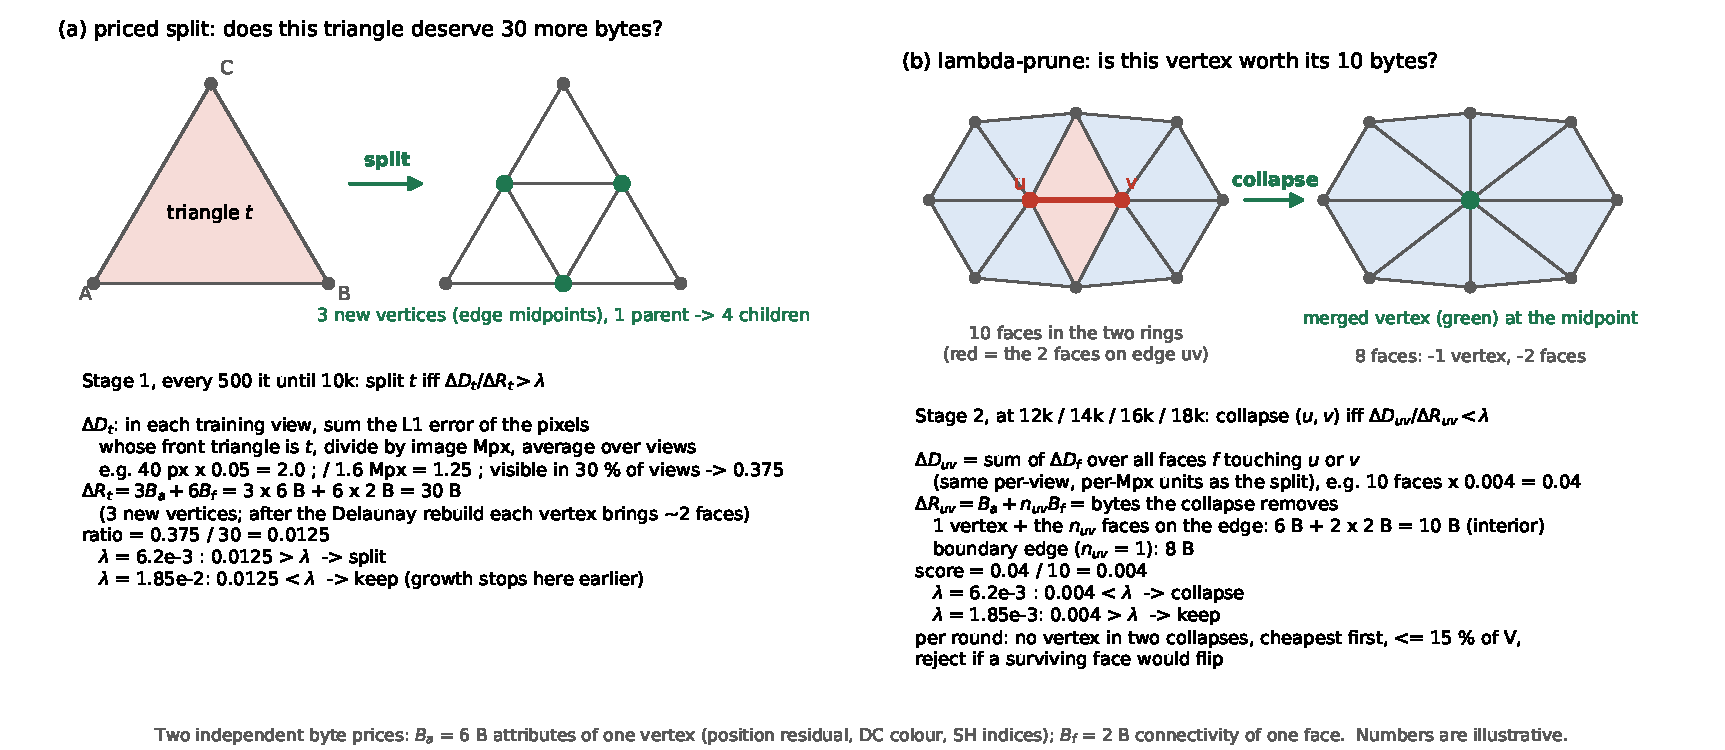
\includegraphics[width=\linewidth]{figures/fig-split-prune-v2.pdf}
\caption{One priced split (a) and one $\lambda$-collapse (b), with illustrative numbers. Both use the same $\lambda$, the same per-face distortion and the same two byte prices $B_a$, $B_f$.}
\label{fig:splitprune}
\end{figure}

\paragraph{Why fixed prices.} $B_a$ and $B_f$ were read once from the codec's stream sizes on a Room mesh and are used unchanged for every scene and every $\lambda$. Over all 44 delivered assets the measured cost is 9.5--13.3\,B per vertex (median 10.8\,B) against the 10\,B the constants give for two faces per vertex. A per-scene price would only rescale that scene's $\lambda$ by at most $1.33\times$, about a quarter of one step of our $\lambda$ grid, whereas a single price keeps $\lambda$ the same exchange rate in every scene.

\textbf{The encoder is not in the training loop.} Its only contribution to training is these two constants; $\Delta R$ is computed from them, never by encoding anything during training. The encoder itself runs once, after iteration 30k, on the frozen model, and cannot influence how the mesh grew.

\subsection{Encoder and decoder}

The encoder takes the finished mesh (positions, faces, 48 SH coefficients per vertex, one opacity scalar) and writes one file.
\begin{itemize}[nosep,leftmargin=*]
  \item \textbf{Positions} are snapped to a $b$-bit grid with $b = \lceil \log_2(\text{extent} / (0.1\cdot\text{median edge})) \rceil$ (14--18 bits per scene), reordered with meshoptimizer for locality, and coded as causal-neighbour residuals.
  \item \textbf{Connectivity} is coded with a cached-edge arithmetic coder after the same reorder; it is the largest stream and is kept lossless.
  \item \textbf{SH} is the lever: the 45 non-DC coefficients of every vertex are replaced by an index into a main dictionary of 4096 vectors plus a residual dictionary of 256, both learnt by $k$-means on the scene and refit for 400 steps against the rendering loss. Indices are coded with a 1-ring context model; the DC term is quantised to 7 bits and zstd-coded.
  \item \textbf{Banks and header} (the two dictionaries, one opacity scalar, grid parameters) are a fixed 0.6\,MB.
\end{itemize}
The decoder is a standalone program with no access to the training data: it reads the five streams, rebuilds positions, faces and per-vertex SH, and hands a standard mesh to any rasteriser. It runs in 2--6\,s on one CPU core. For a Room asset at full growth the file is roughly 16\,MB geometry + 15\,MB SH; the SH dictionary is what makes a 740\,MB FP32 model fit in 31\,MB at $-0.4$\,dB before any growth control.

% =====================================================================
\section{Experiments}
\label{sec:exp}

\paragraph{Setup.} Mip-NeRF~360 (9 scenes) and Tanks \& Temples (truck, train), test split = every 8th view. FP32 = our reproduction of MeshSplatting with the upstream flags (\texttt{--indoor} on room, counter, kitchen, bonsai); it matches the paper within $\pm 0.1$\,dB. MB $= 10^6$ bytes of the delivered file; ratio = FP32 size / delivered size. Each $\lambda$ point is one training run plus one encode; nothing is tuned per scene. LPIPS in our delivered-asset rows is the pipeline convention (inputs in $[-1,1]$), about 0.03 higher than the 3DGS convention used by the paper and by every published baseline; the unified evaluation pass will put all rows on the 3DGS convention.

\subsection{Headline: the RD curve}

\begin{table}[h]
\centering\small
\caption{Dataset means. Mip-NeRF~360, 9 scenes, unless marked T\&T.}
\label{tab:headline}
\begin{tabular}{@{}lrrlr@{}}
\toprule
point & MB & ratio & PSNR / SSIM / LPIPS & $\Delta$PSNR vs FP32 \\
\midrule
FP32 (our reproduction) & 642 & 1$\times$ & 24.81 / 0.731 / 0.309 & -- \\
$\lambda = 6.2\times10^{-4}$ & 26.6 & 24$\times$ & 24.56 / 0.717 / 0.385 & $-0.24$ \\
$\lambda = 1.85\times10^{-3}$ & 20.0 & 32$\times$ & 24.44 / 0.709 / 0.405 & $-0.37$ \\
$\lambda = 6.2\times10^{-3}$ & 9.0 & 72$\times$ & 23.89 / 0.672 / 0.464 & $-0.92$ \\
$\lambda = 1.85\times10^{-2}$ & 4.3 & 151$\times$ & 23.12 / 0.624 / 0.518 & $-1.68$ \\
\midrule
T\&T FP32 & 459 & 1$\times$ & 20.64 / 0.760 / 0.272 & -- \\
T\&T $\lambda = 6.2\times10^{-3}$ & 11.4 & 40$\times$ & 20.52 / 0.737 / 0.358 & $-0.12$ \\
\bottomrule
\end{tabular}
\end{table}

\subsection{Per scene}

\begin{table}[h]
\centering\scriptsize
\caption{Per scene: FP32 model and the four $\lambda$ points. Each cell is MB (ratio) $\cdot$ PSNR.}
\label{tab:perscene}
\setlength{\tabcolsep}{4pt}
\resizebox{\linewidth}{!}{%
\begin{tabular}{@{}lrrllll@{}}
\toprule
scene & FP32 MB & FP32 PSNR & $\lambda\,6.2\mathrm{e}{-4}$ & $\lambda\,1.85\mathrm{e}{-3}$ & $\lambda\,6.2\mathrm{e}{-3}$ & $\lambda\,1.85\mathrm{e}{-2}$ \\
\midrule
room     & 597 & 28.48 & 22.1 (27$\times$) $\cdot$ 28.25 & 12.4 (48$\times$) $\cdot$ 28.02 & 5.4 (110$\times$) $\cdot$ 27.30 & 2.9 (207$\times$) $\cdot$ 26.38 \\
counter  & 520 & 26.48 & 20.7 (25$\times$) $\cdot$ 25.95 & 13.1 (40$\times$) $\cdot$ 25.84 & 6.4 (82$\times$) $\cdot$ 25.32 & 3.3 (155$\times$) $\cdot$ 24.54 \\
kitchen  & 507 & 27.46 & 24.5 (21$\times$) $\cdot$ 27.09 & 16.5 (31$\times$) $\cdot$ 26.89 & 8.0 (63$\times$) $\cdot$ 25.97 & 3.8 (134$\times$) $\cdot$ 24.62 \\
bonsai   & 678 & 28.28 & 24.3 (28$\times$) $\cdot$ 27.89 & 13.2 (52$\times$) $\cdot$ 27.41 & 6.1 (112$\times$) $\cdot$ 26.36 & 3.5 (192$\times$) $\cdot$ 25.36 \\
garden   & 740 & 24.75 & 36.4 (20$\times$) $\cdot$ 24.73 & 24.6 (30$\times$) $\cdot$ 24.50 & 10.2 (73$\times$) $\cdot$ 23.65 & 5.0 (149$\times$) $\cdot$ 22.78 \\
bicycle  & 680 & 23.04 & 31.6 (22$\times$) $\cdot$ 22.99 & 27.0 (25$\times$) $\cdot$ 23.02 & 11.9 (57$\times$) $\cdot$ 22.69 & 5.2 (131$\times$) $\cdot$ 22.08 \\
stump    & 698 & 24.99 & 27.6 (25$\times$) $\cdot$ 24.81 & 21.4 (33$\times$) $\cdot$ 24.71 & 8.9 (79$\times$) $\cdot$ 24.12 & 3.9 (178$\times$) $\cdot$ 23.21 \\
flowers  & 668 & 19.45 & 25.7 (26$\times$) $\cdot$ 19.02 & 24.2 (28$\times$) $\cdot$ 19.07 & 12.0 (56$\times$) $\cdot$ 19.21 & 5.6 (118$\times$) $\cdot$ 18.84 \\
treehill & 692 & 20.39 & 27.0 (26$\times$) $\cdot$ 20.31 & 27.4 (25$\times$) $\cdot$ 20.45 & 11.9 (58$\times$) $\cdot$ 20.38 & 5.1 (136$\times$) $\cdot$ 20.30 \\
truck    & 432 & 22.39 & 27.3 (16$\times$) $\cdot$ 21.78 & 19.3 (22$\times$) $\cdot$ 22.20 & 9.4 (46$\times$) $\cdot$ 22.37 & 4.4 (98$\times$) $\cdot$ 21.64 \\
train    & 485 & 18.90 & 30.1 (16$\times$) $\cdot$ 18.55 & 25.4 (19$\times$) $\cdot$ 18.66 & 13.4 (36$\times$) $\cdot$ 18.68 & 6.4 (76$\times$) $\cdot$ 18.55 \\
\midrule
Mip-360 mean (9) & 642 & 24.81 & 26.6 (24$\times$) $\cdot$ 24.56 & 20.0 (32$\times$) $\cdot$ 24.44 & 9.0 (72$\times$) $\cdot$ 23.89 & 4.3 (151$\times$) $\cdot$ 23.12 \\
T\&T mean (2)    & 459 & 20.64 & 28.7 (16$\times$) $\cdot$ 20.17 & 22.3 (21$\times$) $\cdot$ 20.43 & 11.4 (40$\times$) $\cdot$ 20.52 & 5.4 (85$\times$) $\cdot$ 20.10 \\
\bottomrule
\end{tabular}}
\end{table}

The same $\lambda$ lands at 2.9--6.4\,MB indoors and 5--13\,MB outdoors: the byte budget is decided by scene content, not by a cap. On the hard outdoor scenes (flowers, treehill, truck, train) the two smallest-$\lambda$ points are dominated: growth that the price lets through does not buy test PSNR there, which is exactly what the in-the-loop ablation in Section~\ref{sec:ablation} measures.

\subsection{Same asset, different codecs}

\begin{figure}[h]
\centering
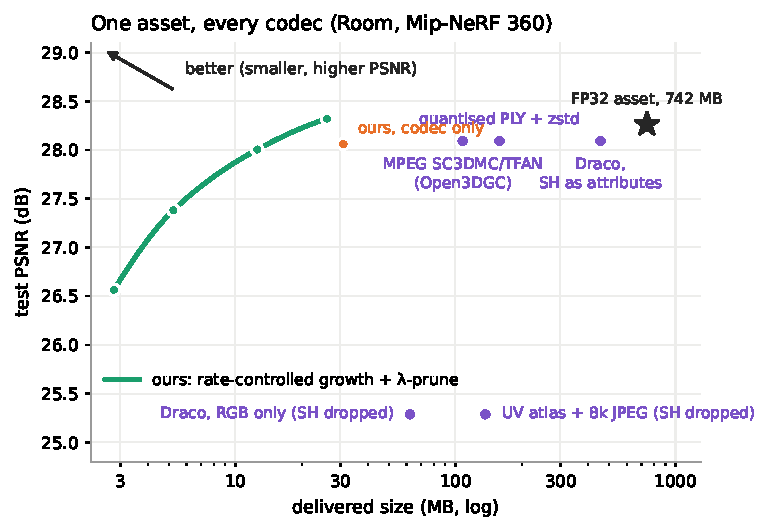
\includegraphics[width=0.9\linewidth]{figures/fig-codecs-room-v2.pdf}
\caption{One FP32 Room asset (3.19\,M vertices, 742\,MB) through generic codecs and through ours. Every point is the same trained model; only the codec differs.}
\label{fig:codecs}
\end{figure}

\begin{table}[h]
\centering\small
\caption{Room, same FP32 asset, different routes.}
\label{tab:codecs}
\resizebox{\linewidth}{!}{%
\begin{tabular}{@{}lrrl@{}}
\toprule
route & MB & PSNR & note \\
\midrule
PLY + zstd & 158.5 & 28.09 & lossless after 8-bit SH quantisation \\
MPEG SC3DMC/TFAN (Open3DGC), SH as 8-bit attributes & 108.0 & $\approx$28.09 & strongest generic row; geometry 19.9 + SH 88.1 \\
Draco, SH as attributes & 456.1 & 28.09 & splits vertices 4.5$\times$ \\
MPEG or Draco geometry + JPEG texture (4k / 8k atlas) & 91--146 & 25.3 & SH dropped, $-3.0$\,dB \\
ours, codec only (level 1.0, no growth control) & 30.9 & 28.06 & 3.5$\times$ smaller than MPEG \\
ours, $\lambda = 2\times10^{-3}$ & 13.7 & 27.99 & 7.9$\times$ smaller than MPEG \\
\bottomrule
\end{tabular}}
\end{table}

Of the 108 $\to$ 31\,MB gain, about 73\,MB comes from replacing per-vertex SH by dictionary indices and about 4\,MB from our geometry streams; swapping only the geometry encoder for MPEG costs 13\,\%. Figure~\ref{fig:codecs} uses the 10/24 Room asset (trained without \texttt{--indoor}); every row in it is on that one asset, so it is internally consistent. Garden behaves the same way (MPEG 126\,MB vs ours 32.5\,MB at equal quality).

\subsection{Against other methods}

\begin{figure}[h]
\centering
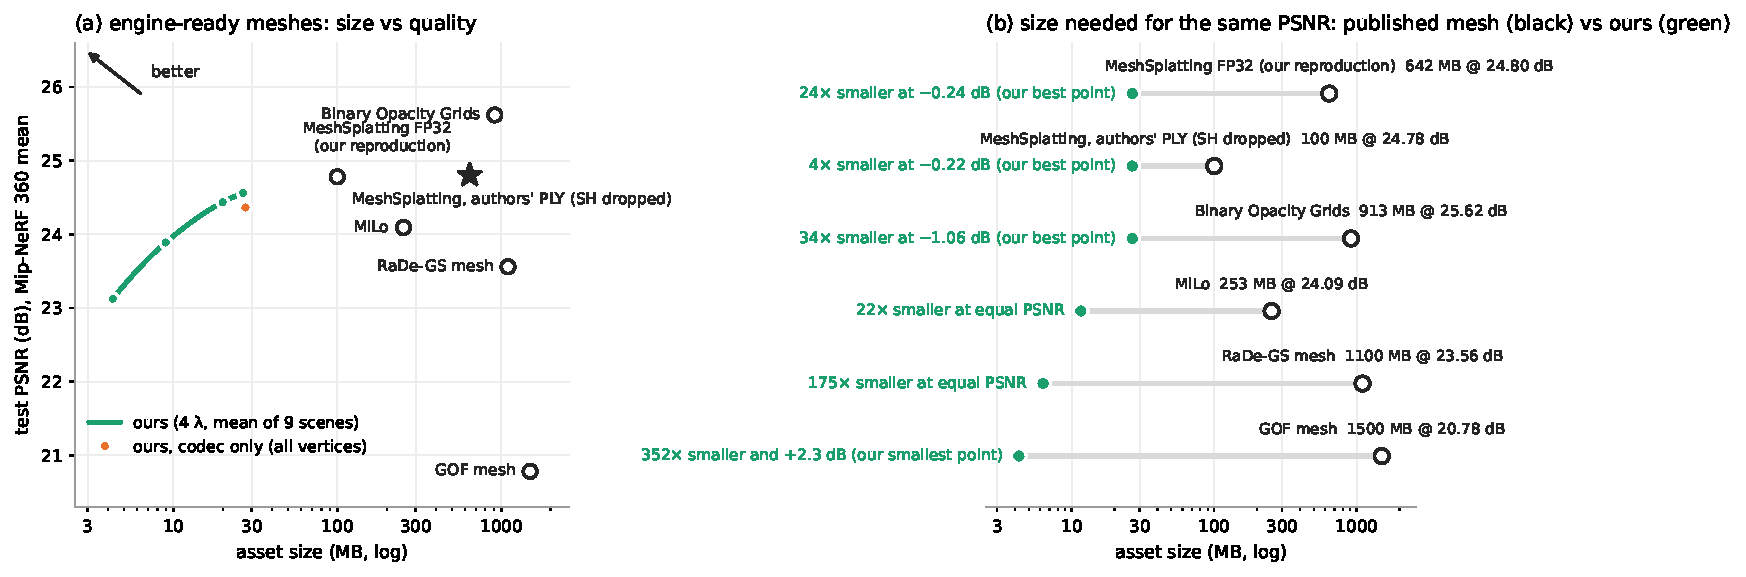
\includegraphics[width=\linewidth]{figures/fig-mesh-class-v2.pdf}
\caption{Engine-ready mesh methods, Mip-NeRF~360 means. (a) size vs PSNR; (b) bytes needed to reach each method's PSNR.}
\label{fig:mesh}
\end{figure}

\begin{figure}[h]
\centering
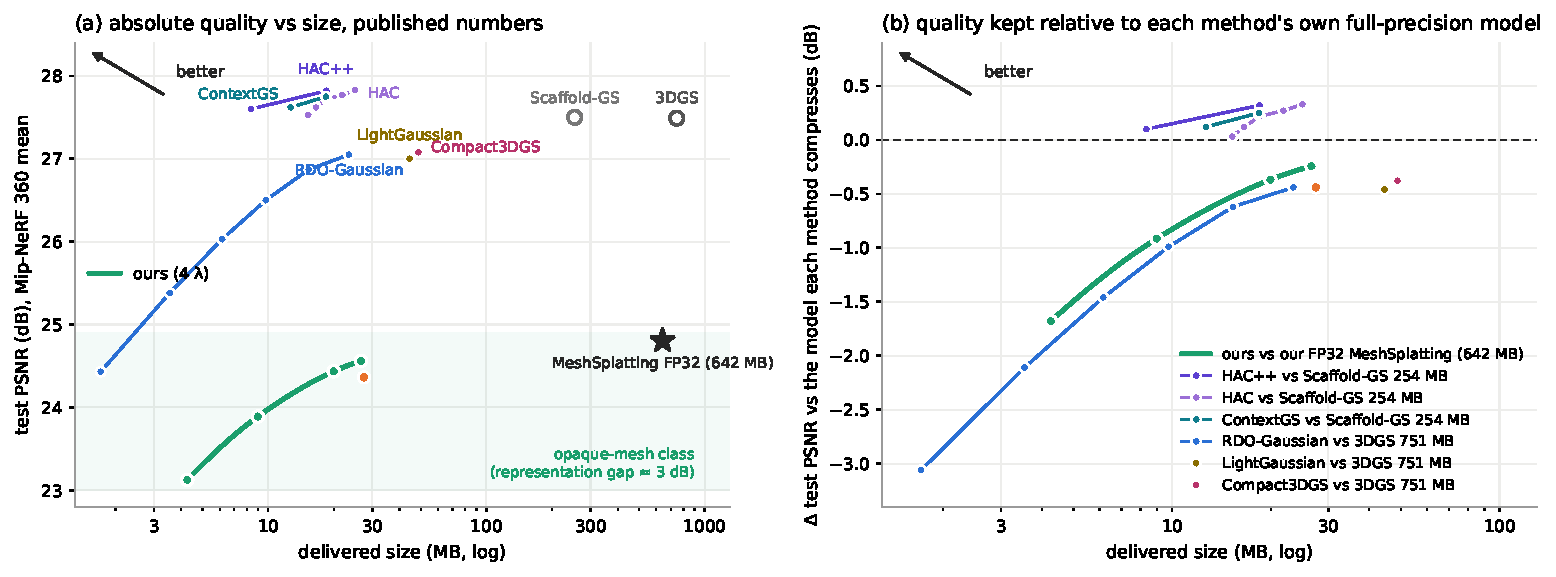
\includegraphics[width=\linewidth]{figures/fig-gauss-class-v2.pdf}
\caption{3DGS-class codecs. (a) absolute numbers; (b) quality retained relative to each method's own full-precision model.}
\label{fig:gauss}
\end{figure}

\begin{table}[t]
\centering\scriptsize
\caption{Cross-method comparison, dataset means, engine-ready mesh methods. Published numbers verbatim; FPS as reported, hardware differs by row; ``--'' = not reported. $\dagger$ pipeline LPIPS convention, $\approx 0.03$ higher than the 3DGS convention of the other rows. $^{a}$ RGB-only PLY, SH dropped. $^{b}$ plus a CPU decode of 2--6\,s; FPS measured on Room (iPhone 17 Pro / MacBook Pro M2 Max, WebGL2).}
\label{tab:cross-mesh}
\setlength{\tabcolsep}{4pt}
\resizebox{\linewidth}{!}{%
\begin{tabular}{@{}llrlrl@{}}
\toprule
method & Mip-360 PSNR / SSIM / LPIPS & MB & T\&T PSNR / SSIM / LPIPS & MB & FPS \\
\midrule
MeshSplatting, paper (2025) & 24.78 / 0.728 / 0.310 & 100$^{a}$ & 20.52 / 0.745 / 0.287 & -- & 220 / 190 (M4) \\
MeshSplatting FP32, our reproduction & 24.81 / 0.731 / 0.309 & 642 & 20.64 / 0.760 / 0.272 & 459 & -- \\
MiLo (SIGGRAPH Asia 2025) & 24.09 / 0.688 / 0.323 & 253 & 21.46 / 0.706 / 0.348 & -- & 170 / 160 (M4) \\
Binary Opacity Grids (SIGGRAPH 2024) & 25.62 / -- / -- & 913 & -- & -- & 927 (desktop) \\
RaDe-GS mesh (2024) & 23.56 / 0.668 / 0.361 & 1100 & 20.51 / 0.659 / 0.344 & -- & OOM on M4 \\
GOF mesh (2024) & 20.78 / 0.573 / 0.465 & 1500 & 21.69 / 0.690 / 0.326 & -- & OOM on M4 \\
\midrule
\textbf{ours, $\lambda = 6.2\times10^{-4}$} & 24.56 / 0.717 / 0.385$^\dagger$ & 26.6 & 20.17 / 0.737 / 0.332$^\dagger$ & 28.7 & 350 phone / 820 laptop$^{b}$ \\
\textbf{ours, $\lambda = 1.85\times10^{-3}$} & 24.44 / 0.709 / 0.405$^\dagger$ & 20.0 & 20.43 / 0.745 / 0.331$^\dagger$ & 22.3 & 350 phone / 820 laptop$^{b}$ \\
\textbf{ours, $\lambda = 6.2\times10^{-3}$} & 23.89 / 0.672 / 0.464$^\dagger$ & 9.0 & 20.52 / 0.737 / 0.358$^\dagger$ & 11.4 & 350 phone / 820 laptop$^{b}$ \\
\bottomrule
\end{tabular}}
\end{table}

\begin{table}[t]
\centering\scriptsize
\caption{Cross-method comparison, dataset means, 3DGS-class methods (not engine-ready meshes). Published numbers verbatim; FPS as reported, hardware differs by row; ``--'' = not reported. Ours (Table~\ref{tab:cross-mesh}) is $\approx 3$\,dB below this class in absolute PSNR; this is the opaque-mesh representation gap, present already in uncompressed MeshSplatting.}
\label{tab:cross-3dgs}
\setlength{\tabcolsep}{4pt}
\resizebox{\linewidth}{!}{%
\begin{tabular}{@{}llrlrl@{}}
\toprule
method & Mip-360 PSNR / SSIM / LPIPS & MB & T\&T PSNR / SSIM / LPIPS & MB & FPS \\
\midrule
3DGS (SIGGRAPH 2023) & 27.46 / 0.812 / 0.222 & 750.9 & 23.69 / 0.844 / 0.178 & 431.0 & 99 (desktop) \\
Scaffold-GS (CVPR 2024) & 27.50 / 0.806 / 0.252 & 253.9 & 23.96 / 0.853 / 0.177 & 86.5 & 135 \\
HAC++ low (2025) & 27.60 / 0.803 / 0.253 & 8.34 & 24.22 / 0.849 / 0.190 & 5.18 & 130--151 \\
HAC++ high (2025) & 27.82 / 0.811 / 0.231 & 18.48 & 24.32 / 0.854 / 0.178 & 8.63 & 130--151 \\
RDO-Gaussian (ECCV 2024) & 27.05 / 0.802 / 0.239 & 23.46 & 23.34 / 0.835 / 0.195 & 12.03 & -- \\
Compact3DGS (CVPR 2024) & 27.08 / 0.798 / 0.247 & 48.80 & 23.32 / 0.831 / 0.201 & 39.43 & -- \\
LightGaussian (NeurIPS 2024) & 27.00 / 0.799 / 0.249 & 44.54 & 22.83 / 0.822 / 0.242 & 22.43 & -- \\
\bottomrule
\end{tabular}}
\end{table}

Inside the engine-ready mesh class we reach MiLo's quality at 22$\times$ fewer bytes, RaDe-GS's at 175$\times$, GOF's at 352$\times$ with $+2.3$\,dB; the authors' own RGB-only PLY (100\,MB) is 4$\times$ larger than our best point and 0.22\,dB higher only because it drops SH entirely. Against 3DGS-class codecs the 3\,dB absolute gap is the opaque-mesh representation gap (MeshSplatting is already 2.7\,dB below 3DGS uncompressed), not a codec gap; the comparable quantity is the quality retained at equal bytes (Figure~\ref{fig:gauss}b), where we retain more than RDO-Gaussian, and the HAC family's $+0.1\ldots+0.3$\,dB comes from Scaffold-GS being more compressible to start with.

\subsection{Ablation: is the rate in the loop worth it?}
\label{sec:ablation}

\begin{figure}[h]
\centering
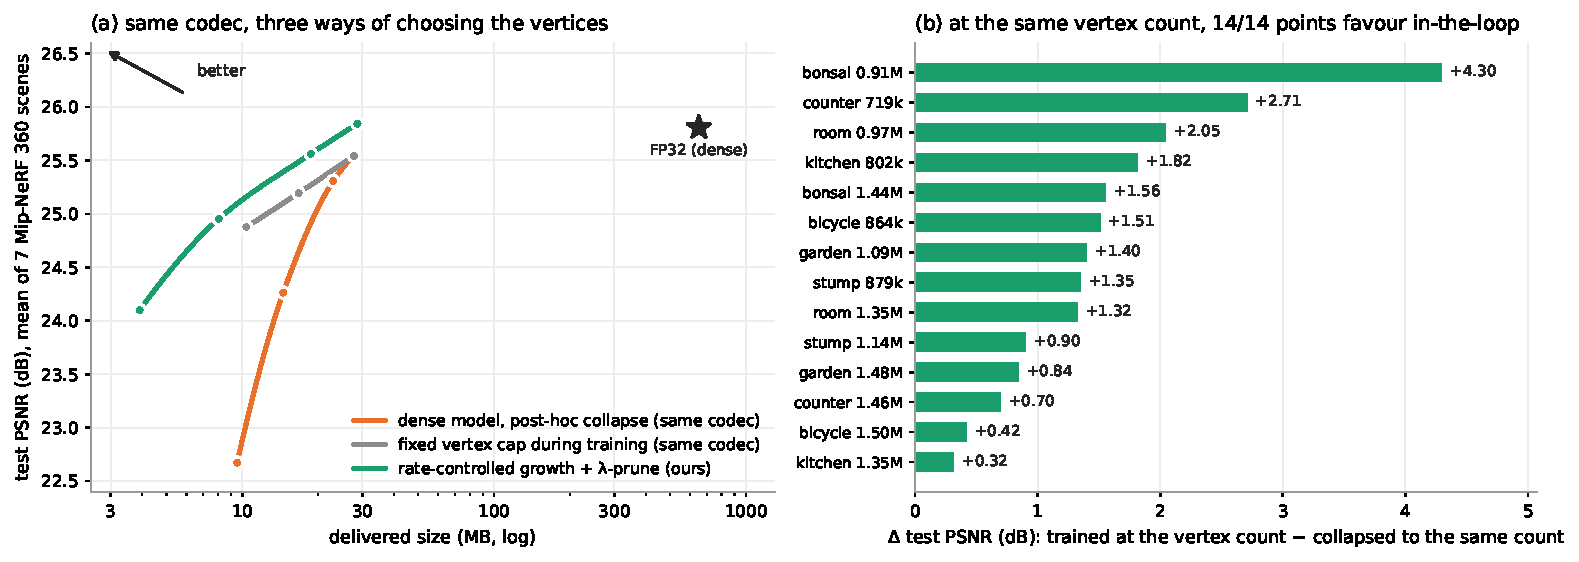
\includegraphics[width=\linewidth]{figures/fig-in-the-loop-v1.pdf}
\caption{Same codec, three ways of choosing vertices (7 Mip-NeRF~360 scenes, older parameter set): post-hoc edge collapse, fixed vertex cap, $\lambda$-growth + prune. (b) At equal vertex count the in-the-loop choice wins on 14 of 14 points.}
\label{fig:loop}
\end{figure}

With the codec held fixed, post-hoc edge collapse to 10\,MB falls to 22.7\,dB mean, training under a fixed vertex cap reaches 24.9\,dB, and $\lambda$-priced growth plus prune reaches 25.0\,dB and keeps going down to 4\,MB. At matched vertex count the in-the-loop choice wins on every scene, by $+0.3$ to $+4.3$\,dB. The prune rounds alone are a small effect ($-8$\,\% bytes at $+0.01$--$0.02$\,dB on Room); the gain is in where growth is allowed to happen.

\subsection{Deployability}

\begin{table}[h]
\centering\small
\caption{Deployability at the $\lambda = 6.2\times10^{-3}$ point. Laptop = MacBook Pro M2 Max (Chrome), phone = iPhone 17 Pro (Safari), WebGL2 viewer, SH degree 3, full capture resolution.}
\label{tab:deploy}
\resizebox{\linewidth}{!}{%
\begin{tabular}{@{}lrrlrll@{}}
\toprule
scene & asset MB & ratio & train min, upstream $\to$ ours & CPU decode s (1 core) & laptop ms (fps) & phone ms (fps) \\
\midrule
room & 5.2 & 142$\times$ & 51 $\to$ 27 (0.52$\times$) & 2.3 & 1.2 (820) & 2.8 (352) \\
garden & 10.2 & 73$\times$ & 49 $\to$ 24 (0.48$\times$) & 4.4 & 1.8 (566) & 6.3 (160) \\
bicycle & 11.9 & 57$\times$ & 41 $\to$ 25 (0.60$\times$) & 5.4 & 1.9 (523) & 6.9 (145) \\
\midrule
11-scene mean & 9.4 & 73$\times$ & 0.57$\times$ & 4.1 & -- & -- \\
\bottomrule
\end{tabular}}
\end{table}

Training is faster than upstream because the mesh stops growing where the price says so; the decoder is a standalone single-core program with no access to the training data.

\subsection{What is still open}
\begin{itemize}[nosep,leftmargin=*]
  \item Indoor assets lose 0.5--0.75\,dB more to the fixed delivery settings (DC 7-bit, 4096 + 256 dictionary) than outdoor ones; a 0.5 GPU-h re-export diagnostic on room and kitchen is planned.
  \item Unified evaluation on the 3DGS LPIPS convention ($\approx$ 3 GPU-h) and MPEG rows for the remaining nine scenes (CPU) are pending; neither changes the ordering above.
\end{itemize}

\end{document}
